%	PACKAGES AND OTHER DOCUMENT CONFIGURATIONS

\documentclass[11pt, a4paper]{article} % 10pt font size (11 and 12 also possible), A4 paper (letterpaper for US letter) and two column layout (remove for one column) Use additional titlepage argument to generate this
%\documentclass[12pt, a4paper,twocolumn,titlepage]{article}

%%%%%%%%%%%%%%%%%%%%%%%%%%%%%%%%%%%%%%%%%
% Wenneker Article
% Structure Specification File
% Version 1.0 (28/2/17)
%
% This file originates from:
% http://www.LaTeXTemplates.com
%
% Authors:
% Frits Wenneker
% Vel (vel@LaTeXTemplates.com)
%
% License:
% CC BY-NC-SA 3.0 (http://creativecommons.org/licenses/by-nc-sa/3.0/)
%
%%%%%%%%%%%%%%%%%%%%%%%%%%%%%%%%%%%%%%%%%

%----------------------------------------------------------------------------------------
%	PACKAGES AND OTHER DOCUMENT CONFIGURATIONS
%----------------------------------------------------------------------------------------

\usepackage[english]{babel} % English language hyphenation

\usepackage{microtype} % Better typography

\usepackage{verbatim} % Allows mulitline commenting

\usepackage{amsmath,amsfonts,amsthm} % Math packages for equations

\usepackage[svgnames]{xcolor} % Enabling colors by their 'svgnames'

\usepackage[hang, small, labelfont=bf, up, textfont=it]{caption} % Custom captions under/above tables and figures

\usepackage{subcaption}

\usepackage{booktabs} % Horizontal rules in tables

\usepackage{lastpage} % Used to determine the number of pages in the document (for "Page X of Total")

\usepackage{graphicx} % Required for adding images

\usepackage{enumitem} % Required for customising lists
\setlist{noitemsep} % Remove spacing between bullet/numbered list elements

\usepackage{sectsty} % Enables custom section titles
\allsectionsfont{\usefont{OT1}{phv}{b}{n}} % Change the font of all section commands (Helvetica)

\usepackage{siunitx}

%----------------------------------------------------------------------------------------
%	MARGINS AND SPACING
%----------------------------------------------------------------------------------------

\usepackage{geometry} % Required for adjusting page dimensions

\geometry{
	top=1cm, % Top margin
	bottom=1.5cm, % Bottom margin
	left=2cm, % Left margin
	right=2cm, % Right margin
	includehead, % Include space for a header
	includefoot, % Include space for a footer
	%showframe, % Uncomment to show how the type block is set on the page
}

\setlength{\columnsep}{7mm} % Column separation width

%----------------------------------------------------------------------------------------
%	FONTS
%----------------------------------------------------------------------------------------

\usepackage[T1]{fontenc} % Output font encoding for international characters
\usepackage[utf8]{inputenc} % Required for inputting international characters

\usepackage{XCharter} % Use the XCharter font

%----------------------------------------------------------------------------------------
%	HEADERS AND FOOTERS
%----------------------------------------------------------------------------------------

\usepackage{fancyhdr} % Needed to define custom headers/footers
\pagestyle{fancy} % Enables the custom headers/footers

\renewcommand{\headrulewidth}{0.0pt} % No header rule
\renewcommand{\footrulewidth}{0.4pt} % Thin footer rule

\renewcommand{\sectionmark}[1]{\markboth{#1}{}} % Removes the section number from the header when \leftmark is used

%\nouppercase\leftmark % Add this to one of the lines below if you want a section title in the header/footer

% Headers
\lhead{} % Left header
\chead{\textit{\thetitle}} % Center header - currently printing the article title
\rhead{} % Right header

% Footers
\lfoot{} % Left footer
\cfoot{} % Center footer
\rfoot{\footnotesize Page \thepage\ of \pageref{LastPage}} % Right footer, "Page 1 of 2"

\fancypagestyle{firstpage}{ % Page style for the first page with the title
	\fancyhf{}
	\renewcommand{\footrulewidth}{0pt} % Suppress footer rule
}

%----------------------------------------------------------------------------------------
%	TITLE SECTION
%----------------------------------------------------------------------------------------

\newcommand{\authorstyle}[1]{{\large\usefont{OT1}{phv}{b}{n}\color{NavyBlue}#1}} % Authors style (Helvetica)

\newcommand{\institution}[1]{{\footnotesize\usefont{OT1}{phv}{m}{sl}\color{Black}#1}} % Institutions style (Helvetica)

\usepackage{titling} % Allows custom title configuration

\newcommand{\HorRule}{\color{SteelBlue}\rule{\linewidth}{1pt}} % Defines the gold horizontal rule around the title

\pretitle{
	\vspace{-30pt} % Move the entire title section up
	\HorRule\vspace{10pt} % Horizontal rule before the title
	\fontsize{32}{36}\usefont{OT1}{phv}{b}{n}\selectfont % Helvetica
	\color{Navy} % Text colour for the title and author(s)
}

\posttitle{\par\vskip 15pt} % Whitespace under the title

\preauthor{} % Anything that will appear before \author is printed

\postauthor{ % Anything that will appear after \author is printed
	\vspace{10pt} % Space before the rule
	\par\HorRule % Horizontal rule after the title
	\vspace{20pt} % Space after the title section
}

%----------------------------------------------------------------------------------------
%	ABSTRACT
%----------------------------------------------------------------------------------------

\usepackage{lettrine} % Package to accentuate the first letter of the text (lettrine)
\usepackage{fix-cm}	% Fixes the height of the lettrine

\newcommand{\initial}[1]{ % Defines the command and style for the lettrine
	\lettrine[lines=3,findent=4pt,nindent=0pt]{% Lettrine takes up 3 lines, the text to the right of it is indented 4pt and further indenting of lines 2+ is stopped
		\color{NavyBlue}% Lettrine colour gold DarkGoldenRod
		{#1}% The letter
	}{}%
}

\usepackage{xstring} % Required for string manipulation

\newcommand{\lettrineabstract}[1]{
	\StrLeft{#1}{1}[\firstletter] % Capture the first letter of the abstract for the lettrine
	\initial{\firstletter}\textbf{\StrGobbleLeft{#1}{1}} % Print the abstract with the first letter as a lettrine and the rest in bold
}

%	BIBLIOGRAPHY

\usepackage[backend=biber,style=phys,natbib=true,doi=false]{biblatex} 
%Can equally use numeric citation style without extra phys packaging (but doesn't change capitalisation), or authoryear for alphabetical listing without the codes (resembles APA)

%\addbibresource{references.bib} % The filename of the bibliography

\usepackage[autostyle=true]{csquotes} % Required to generate language-dependent quotes in the bibliography

%    APPENDICES

\usepackage[title]{appendix} %in appendix


 % Specifies the document structure and loads requires packages
\graphicspath{{"/Users/kit gallagher/Documents/Research Review/Report/Figures"}}
\newcommand*{\subscript}[1]{\ensuremath{_\textrm{{\scriptsize #1}}}}

%	ARTICLE INFORMATION

\title{Simulating Liquid Crystals}

%\author{
	%\authorstyle{Christopher Gallagher}}
\author{\authorstyle{Kit Gallagher} 
	%\institution{University of Cambridge \\
	\institution{Supervisors: Prof Erika Eiser, Mr Jiaming Yu}}
% Example of a one line author/institution relationship
%\author{\newauthor{John Marston} \newinstitution{Universidad Nacional Autónoma de México, Mexico City, Mexico}}

\date{\today} % Add a date here if you would like one to appear underneath the title block, use \today for the current date, leave empty for no date
\usepackage[english]{babel}
\usepackage{tabularx}
%\renewcommand{\thefootnote}{\roman{footnote}}  %use roman lettering for footnotes instead
%\usepackage[backend=biber,doi=false]{biblatex}
\addbibresource{reportreferences.bib}
\AtBeginBibliography{\small}
%----------------------------------------------------------------------------------------
\begin{document}

\maketitle % Print the title

\thispagestyle{firstpage} % Apply the page style for the first page (no headers and footers)

%	ABSTRACT

\lettrineabstract{The specificity of DNA base-pair interactions gives considerable functional control in the design of anisotropic nano-particles, enabling the formation of liquid crystal phases. This project aims to study the liquid phase behaviour of such non-conventional liquid crystal molecules, with a particular focus on the novel `nunchuck' structure - two rigid rods connected via a flexible linker. The Eiser Group have previously considered intra-molecular interaction potentials at the single-nucleotide level for a single DNA nanoparticle, and I am now implementing these potentials in larger, more coarse-grained models of multiple nanoparticles, through open-source software LAMMPS (Large-scale Atomic/Molecular Massively Parallel Simulator). Such systems are expected to form smectic (layered) phases at high volume fractions.} 

%The specificity of DNA base pair interactions allows the design of anisotropic nano-particles such as rods, triangles and many other shapes. Such anisotropy is a pre-requisite to form liquid crystalline structures. The exciting part is that because we can now make new shapes we expect to obtain completely new liquid crystalline symmetries. Based on oxDNA, a semi-coarse-grained, freely available simulation package that can provide the topological and stability criteria of any DNA nano-particle, the Eiser group developed a more coarse-grained model to simulate large numbers of these mesogens such that their phase-behavior can be studied.


%	ARTICLE CONTENTS
\section{Introduction}
Short DNA strands are observed to form liquid crystalline phase structures at sufficiently high concentrations. This project uses a course-grained model based on LAMMPS \cite{Xing2019} to study the phase behaviour of ‘nunchuks’, which are two rigid rods of double stranded (ds-) DNA, connected via a flexible linker of single stranded (ss-) DNA. This linker allows the configuration to vary from fully stretched to folded.  

The techniques developed here may also be applied to more complex DNA origami to find the phase behaviour of such structures. Through consideration of which simple DNA structures may give rise to Liquid Crystal behaviour, and how they may be implemented in DNA origami, we develop techniques ultimately key in nano-structure self-assembly.

This technology may also be applied to displays, with new phases being applicable for different colour development/better colour control. Very little is known about the potential of DNA here, however its tunability and controllability at the nano-level suggests it could be significant. This is also relevant for light harvesting; conventional solar cells are limited by their well-defined, narrow band gap, which only absorbs from a small part of the black body spectrum. Optically active materials are therefore required to down/upconvert the incoming light here to improve the efficiency.

In Section \ref{LitReview}, this report outlines the basic theory behind liquid crystals, gives a brief background behind the experimental development of liquid crystalline phases of DNA, and the previous simulation work in this area. The simulation processes used in the project are then detailed in Section \ref{ProjPlan}, and the future direction for research outlined.


\section{Background} \label{LitReview}
\subsection{Liquid Crystals}
First identified as an intermediary phase between solids and liquids in 1888 by Friedrich Reinitzer \cite{Reinitzer1888}, the fundamental classes of liquid crystals were characterised in the following decades by Georges Friedel (among others) \cite{Friedel1922}. Research into the applications of liquid crystals only became widespread in the 1960s however, initiated by the seminal research of George William Gray \cite{Gray1962}, and culminating Heilmeier's development of the first liquid crystal display \cite{Heilmeier1969, Heilmeier1968}. Later, in 1991, Pierre-Gilles de Gennes  received the Nobel Prize in physics ``\textit{for discovering that methods developed for studying order phenomena in simple systems can be generalized to more complex forms of matter, in particular to liquid crystals and polymers}'' \cite{deGennes1992}.

In the most general sense, liquid crystals are states of matter displaying properties between those of conventional liquids and solid crystals. For this reason, they are also known as mesomorphic phases, with individual molecules being referred to as mesogens, and these terms will be used interchangeably through this report. While solid crystals display long range periodic order in three dimensions (and isotropic liquids in none), liquid crystals have a degree of long range order in some (but not all) spatial dimensions. There are three fundamental classes \cite{DeGennes1993}, visualised in Figure \ref{fig:lcphasescropped}.

\begin{itemize}
	\item \textbf{Nematic:} No positional order, but orientational order as molecules\footnotemark \ tend to point in the same direction.
	\item \textbf{Smectic:} One dimensional positional order, so has the appearance of 2D liquid layers separated by a well defined spacing.
	\item \textbf{Columnar:} Two dimensional positional order, so has the appearance of an 2D array of liquid tubes.
\end{itemize}

\footnotetext{It should be noted that only achiral molecules may form nematic phases; chiral molecules form an equivalent cholesteric (or `twisted-nematic') phase. This is particularly relevant to the consideration of DNA; a chiral molecule.}

\begin{figure} [h!]
	\centering
	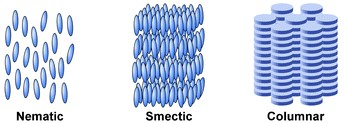
\includegraphics[width=0.7\linewidth]{Figures/lc_phases_cropped}
	\caption{Representation of the three liquid crystal phase classes, reproduced from Kato et al. \cite{Kato2007} with permission. Note the distinct layers in the smectic and columnar phases, and the different class of molecule in the columnar phase.}
	\label{fig:lcphasescropped}
\end{figure}


It should be noted that the higher order phases (smectic and columnar) also display orientational order throughout the body. This is fundamental to the formation of liquid crystals, and so (almost) all mesogenic molecules are anisotropic. We will see later that the degree of anisotropy affects the stability of different phases. 

As is visible in Figure \ref{fig:lcphasescropped}, this anisotropy can come in different forms. `Rod-like' molecules (where anisotropy is in the form of one elongated axis) are the oldest, and most popular, form of liquid crystal. They favour the formation of nematic and smectic phases, and will form the focus of this report. Alternatively, disk shaped (discotic) molecules (discovered by Chandrasekhar in 1977 \cite{Chandrasekhar1977}) have one compressed axis, and favour the formation of other nematic or columnar phases. In 1987, Lam subsequently predicted the existence of a sub-class of `bowlic' molecules which break the up-down symmetry of discotic molecules \cite{LinLei1988}, which were subsequently found experimentally \cite{Zimmermann1985, Malthete1985}.

Liquid crystals can also be categorised by the driving force behind the transition. Smaller molecules tend to undergo thermally driven phase transitions, and so form different thermotropic phases in different temperature ranges. By contrast, larger molecules tend to undergo lyotropic, or concentration driven phase transitions \cite{DeGennes1993}.

\subsection{Onsager Theory} \label{Onsager}
Onsager predicted a simple model of lyotropic phase transitions \cite{Onsager1949}, which will be employed in this project. Rod-like particles are modelled as rigid rods, with an excluded volume preventing interpenetration/overlap. The interaction potentials between molecules are neglected, and only the configurational entropy of the system considered. Fundamentally, the confinement of rods to parallel orientations (such as in the nematic phase) leads to a decrease in orientational entropy, but an increase in positional entropy (as each rod takes up less space). At sufficiently high concentrations, the positional entropy will dominate, and the system undergo a phase transition from isotropic to nematic. 

It can be shown that the critical volume fraction at transition is approximately $4r/L$, where $r$ is the radius of the rigid rod, and $L$ is the length. The full derivation is rather involved, so will not be replicated here, but is detailed by Doi et al. \cite{Doi1988}. However, the key results are that the isotropic--nematic phase transition occurs at lower concentrations for mesogens with greater aspect ratios, and requires a minimum aspect ratio of $L/r = 4$ to occur.

\subsection{DNA as a Liquid Crystal} 
%zhao2019 is useful review and gives onsager theory
%nakata is beyond onsager theory
%wang2018 gives useful section on history
Lyotropic liquid-crystalline phases are very common in living systems, from cellular membranes to fibroblast structures \cite{Stewart1966, Rey2013}. In vitro, many biochemical molecules such as cellulose, peptides, and protein assemblies have also been shown to form liquid crystal states \cite{Zhao2019}. With respect to the mesogenic behaviour of DNA, Luzzati et al. first observed a columnar phase in a condensed DNA solution in 1959 (only 6 years after the discovery of the double-helix structure), and Robinson pioneered the development of the twisted-nematic phase in 1961 \cite{Luzzati1959, Robinson1961}. 

Subsequent work by Strzelecka et al. has demonstrated experimentally that DNA molecules can form precholestric, cholestric and smectic phases (in order of increasing concentration) though lyotropic phase transitions \cite{Strzelecka1988}. 
Returning to Onsager's theory, with the known dimensions of DNA we find that that the minimum base pair length required to obtain liquid crystalline phase behaviour is 24 base pairs \cite{Bolhuis1997}. However this limit has been broken experimentally by Nakata et al. \cite{Nakata2007, Zanchetta2008}, which they suggest is a result of monomer stacking through end-to-end adhesion to form the larger mesogens required.

These techniques may be applied to developing DNA origami, the process whereby complex nano-structures are constructed out of DNA molecules. Though a greater understanding of the phase behaviour of DNA nanoparticles, we may inform design of more complex structures, and develop colloidal self-assembly processes. These techniques may have applications in fields as diverse as biophysics, photonics, structural biology, and synthetic biology \cite{Nummelin2018, Praetorius2017, Bathe2017}.

\subsection{Previous Simulation Work} \label{PrevWork}
Computational work may be implemented over a broad spectrum of coarse-graining (a process whereby microscopic degrees of freedom are integrated over to reduce the computational costs of a simulation at the cost of lower model resolution), where the base unit of the simulation ranges from single atoms to large bulk molecules \cite{Inglfsson2013, Potoyan2012}. Atomistic models, such as CHARMM \cite{MacKerell1995} and AMBER \cite{SalomonFerrer2012}, offer the greater level of detail, but are limited by computational cost beyond small (>30 base pairs) models \cite{Cheatham2004}. In contrast, bead-spring polymer models (with up to 3000 base pairs per bead) may obtain bulk material properties at significantly lower computational expense \cite{Michieletto2016}.

Such models have been applied specifically to DNA nunchucks by Salamonczyk et al. \cite{Salamonczyk2016} to suggest the existence of smectic phases, however this is limited by the level of coarse-graining applied, as the artificial interaction potentials considered have no basis in their physical origin. This project work builds on this research, by applying a intra-molecular potential derived by single nucleotide simulations of the nunchuck molecule by Jiaming Yu (within the Eiser Group) using OxDNA, a lower-level coarse grained model that accurately represents the physical properties of single and double stranded DNA \cite{OxDNA}.

My work is based on a coarse-grained model developed by Xing et al. \cite{Xing2019} to consider Y-shaped nanoparticles constructed from DNA, and utilises LAMMPS \cite{LAMMPS} software to model dense systems of these nunchuck nano-particles. This approach applies the increased resolution of the single nucleotide OxDNA model to larger systems of many such molecules, to provide a better predictor of this system's experimental phase behaviour.

%xing description of oxdna vs ball and spring models
\section{Project Plan} \label{ProjPlan}
\subsection{Literature Review}
I have completed an initial literature review, which is reproduced in part within Section \ref{LitReview}. This had three roles:

\begin{itemize}
	\item Understand the history and theory of liquid crystals 
	\item Consider the formation of liquid crystal phases by DNA mesogens
	\item Review the current simulations methods applicable to DNA nano-particles
\end{itemize}

\subsection{LAMMPS Software}
As introduced in Section \ref{PrevWork}, the bulk of the computational work for this project will be completed using the LAMMPS software. LAMMPS (Large-scale Atomic/Molecular Massively Parallel Simulator) is a medium coarse-grained, classical molecular dynamics code developed to replicate  solid-state materials and soft matter mesoscopic systems \cite{Plimpton1995, LAMMPS}. 

\subsubsection{Building Nunchucks}
The nunchucks are formed of two rigid rods of ds-DNA, connected via a flexible linker of ss-DNA, and the complete nunchuck is modelled as a rod of 60 base pairs long. With the standard values for DNA of radius $r = 2$nm and length (per base pair) of $l=0.33$nm, we obtain an aspect ratio of 10 for this rod. It is worth noting that this is above Onsager's limit (discussed in Section \ref{Onsager}) for the formation of a nematic phase; this will be tested in Section \ref{Future}. Within LAMMPS, this is expressed as ten spherical balls (aspect ratio 1) bound rigidly together in a linear structure. It is worth noting that the persistence length of DNA is around 50nm \cite{Garcia2007}, so the approximation of perfect rigidity is valid over the length-scale of the molecule.

\begin{figure} [h!]
	\centering
	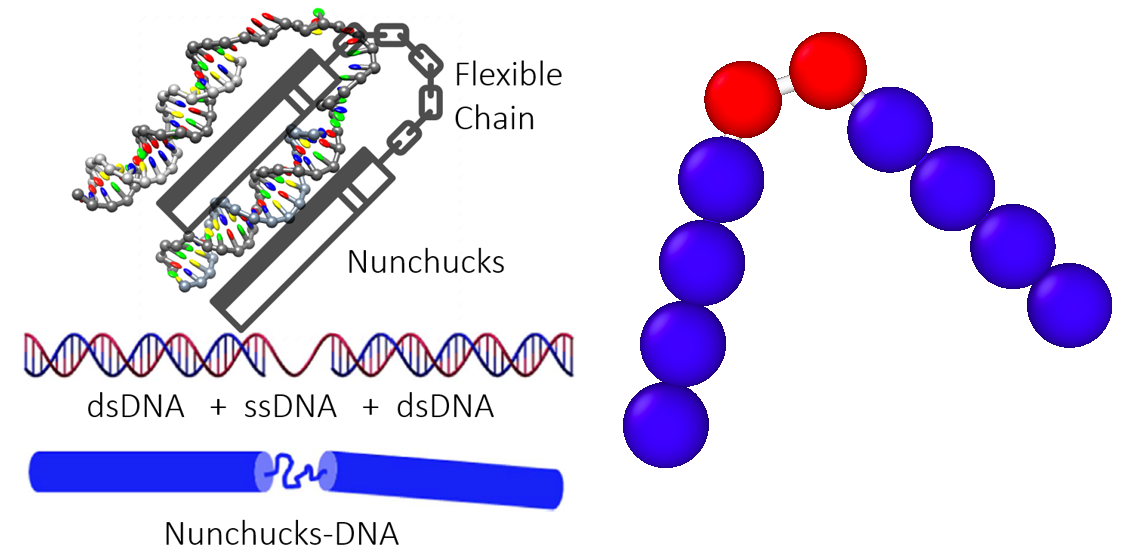
\includegraphics[width=0.7\linewidth]{Figures/nunchucks_combined}%nunchucks_artist}
	\caption{Depictions of the relation between the DNA mesogen and the nunchucks analogy. Note the appearance of the flexible ss-DNA linker between the rigid ds-DNA rods, and the representation within LAMMPS on the right. Figure created by Jiaming Yu (Eiser Group).}
	\label{fig:nunchucks_artist}
\end{figure}

We then introduce a flexible section in the middle of this molecule, by removing one strand of DNA across a region of central base pairs. The number of base pairs affected determines the rigidity of the resulting nunchuck, and varies between about 3 base pairs (minimal bending possible) to 20 base pairs (almost complete flexibility). Within LAMMPS, the central bond (between balls 5 and 6) is modelled as having a reduced rigidity, so the molecule can bend at this point, as displayed in Figure \ref{fig:nunchucks_artist}. Ultimately, a bending potential derived from the OxDNA model may be implemented here, to accurately represent the known physical behaviour of the nunchucks.


%dePablo is a useful review in this area.\ \cite{dePablo2011}

\subsubsection{Running Simulations}
To run simulations within LAMMPS, a file containing the initial positions of each ball must be generated within the simulation region (a cuboid with periodic boundary conditions). This is non-trivial to generate for large numbers of mesogens, as molecules must be placed randomly without overlap, to prevent any initial order affecting the formation of ordered phases, and I am grateful to Iria Pantazi for writing a python script to automate this process. 

To generate a highly concentrated initial state, it is not possible to directly write down particle positions as above, due to the high probability of overlapping molecules in any random position. Instead a more dilute system is generated, and then simulate a constant enthalpy shrinking process (using a Nose-Hoover thermostat \cite{Shinoda2004}) through LAMMPS to increase the mesogen concentration. The system is then allowed to equilibrate over a fixed time duration, while conserving system energy and volume. Both processes also employ a Langevin thermostat to ensure constant temperature throughout.

The position and velocity of every ball may be output at desired time-steps, and the visualisation software Ovito \cite{Ovito} has been employed to animate the molecule motion over the simulation period. Key thermodynamic variables, such as pressure and internal energy, may also be output at regular intervals; I have written python code to extract and plot this data.

\subsubsection{Testing Models}
Initial testing was focused on the known phase behaviour of well studied systems, with initial consideration of rigid rod mesogens (with no bending). These are expected to follow Onsagers theory (Section \ref{Onsager}), and I hope to observe phase transitions in the predicted regions.

Phase diagrams may be plotted by running multiple LAMMPS simulations at different final volumes, to so that lyotropic phase transformations may be observed between different mesogen concentrations. In rigid rods, this may be done through the order parameter; although in more complex systems where this is less well defined, the equilibrium values of other thermodynamic variables (such as pressure or internal energy) may be used to identify the phase transition.

\subsection{Project Direction} \label{Future}
The fundamental aim of this project is to identify smectic phase formation in concentrated nunchuck systems. This requires implementation of the flexible linkage potential into the LAMMPS model, and simulations over a sufficient number of mesogens. The phase transition may be characterised by a number of equilibrium thermodynamic variables, but geometric methods to characterise the phase transition (through the extension of the conventional order parameter to non-linear, flexible mesogens) will also be considered. It is possible that the local correlation of the opening angle (or the direction of the vector bisecting the angle) may be suitable here, but this has not yet been tested.
 
Further work may investigate the effects of a number of variables:
\begin{itemize}
	\item The number of base pairs in the ss-DNA region (i.e. the rigidity of the flexible connector)
	\item The effect of varying the aspect ratio of the rigid rods
	\item The implications of unequal arm lengths, where the molecule is no longer symmetric about the centre of the flexible linker
\end{itemize}

The depth of these investigations will depend on progress with earlier simulation work, and the computational resources available.

%\clearpage
\vspace{2cm}
\noindent \begin{tabular}{@{}p{.55in}p{4in}@{}}
	Signed: & \hrulefill \\
	& Kit Gallagher \textit{(Part III Student)} \\
\end{tabular}

\vspace{1.5cm}
\noindent \begin{tabular}{@{}p{.55in}p{4in}@{}}
	Approved: & \hrulefill \\
	& Professor Erika Eiser \textit{(Project Supervisor)} \\
\end{tabular}
%sign with smallpdf.com


%\clearpage
\printbibliography

\end{document}


%%%%%%%%%%%%%%%%%%%%%%%%%%%%%%%%%%%%%%%%%
% Wenneker Article
% LaTeX Template
% Version 2.0 (28/2/17)
%
% This template was downloaded from:
% http://www.LaTeXTemplates.com
%
% Authors:
% Vel (vel@LaTeXTemplates.com)
% Frits Wenneker
%
% License:
% CC BY-NC-SA 3.0 (http://creativecommons.org/licenses/by-nc-sa/3.0/)
%
%%%%%%%%%%%%%%%%%%%%%%%%%%%%%%%%%%%%%%%%%
